\chapter{Lattices and Structure Definitions}
\adjustmtc
\minitoc
\section{Dual Lattice}
In this section we define the notian of the \textit{dual} of a lattice and see some of its applications.
\begin{definition}(Dual Lattice)
For a full-rank lattice $\Lambda$ we define its dual lattice (sometimes known
as the reciprocal lattice):
\begin{equation}
\Lambda^* = \left\{y\in\mathbb{R}^n\vert \forall x \in \Lambda, \langle x,y
\rangle \in \mathbb{Z}\right\}.
\end{equation}
In general, we define:
\begin{equation}
  \Lambda^* = \left\{y\in\mathrm{span}(\Lambda)\vert\forall x\in \Lambda,
  \langle x,y \rangle\in \Lambda\right\}.
\end{equation}
\end{definition}
In other words, the dual of $\Lambda$ is the set of all points (in the span of
$\Lambda$) whose inner product with any of the points in $\Lambda$ is an
integer. As we will show later, $\Lambda^*$ is indeed a lattice, as the name
suggests.

\begin{example}
  The lattice of integer points satisfies $(\mathbb{Z}^n)^*=\mathbb{Z}$ (and
  hence can be called self-dual). Similarly, $(2\mathbb{Z}^n)^*
  = \frac{1}{2}\mathbb{Z}^n$, and this gives some justification to the name 
  reciprocal lattice.
\end{example}
\par From the above definition, we have the following geometrical
interpretation of the dual lattice. For any vector $x$, the set of all
points whose inner product with $x$ is integer forms a set of hyperplanes
perpendicular to $x$ and separated by distance $1/||x||$. Hence, any vector
$x$ in a lattice $\Lambda$ imposes the constraint that all points
in $\Lambda^*$ lie in one of the hyperplanes defined by $x$. The next figure
tries to illustrate that notion.
\begin{figure}[h!]
  \centering
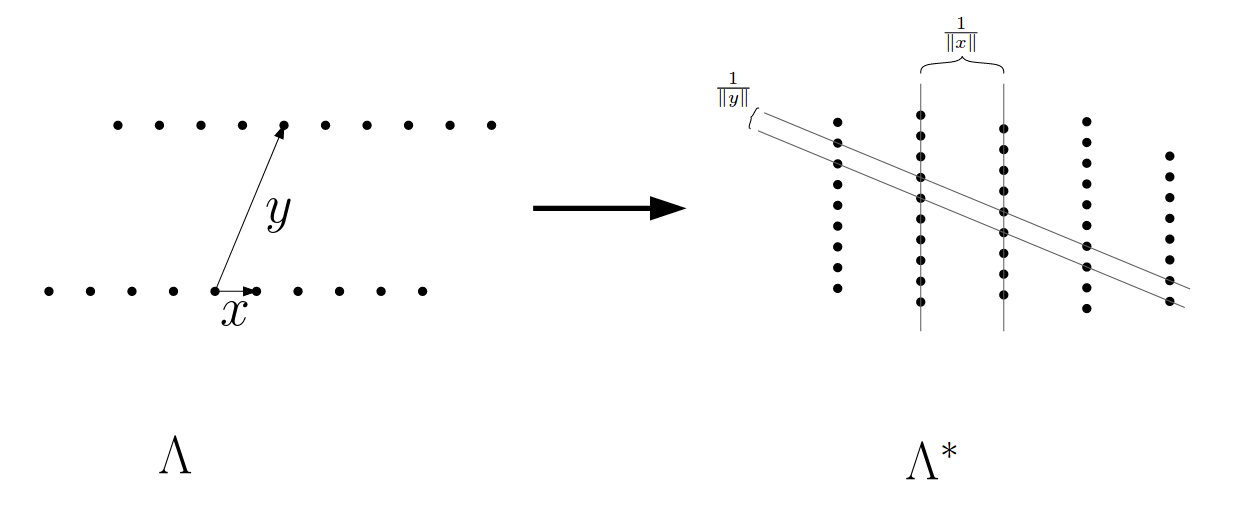
\includegraphics[width=0.8\textwidth]{Images/duallattice.png}
  \caption{A lattice and its dual}
\end{figure}
\begin{definition}(Dual Basis)
  For a basis $B=(b_1,\dots,b_n)\in\mathbb{R}^{m\times n}$, define the dual
  basis $D=(d_1,\dots,d_n)\in \mathbb{R}^{m\times n}$ as the unique basis that
  satisfies
  \begin{itemize}
    \item $\mathrm{span}(D) = \mathrm{span}(B)$
    \item $B^TD = \mathbb{I}$
  \end{itemize}
\end{definition}
\par The second condition can be interpreted as saying that $\langle b_i,
d_j\rangle = \delta_{ij}$ where $\delta_{ij}$ is the usual Kroneker delta. It
is not hard to check that $D$ is indeed unique. In fact, for the case of
a full-rank lattice, $D$ is given by $(B^T)^{-1}$; in general, we get $D=B(B^T
B)^{-1}$ (and we could use this as our definition of a dual basis).
\par In the next claim, we show that if $B$ is a basis of a lattice $\Lambda$,
then the dual basis of $B$ is a basis of $\Lambda^*$. In particular, this shows
that $\Lambda^*$ is indeed a lattice.
\begin{proposition}
  If $D$ is the  dual basis of $B$ then $(\mathcal{L}(B))^* = \mathcal{L}(D)$.
\end{proposition}
\begin{proof}
  We first show that $\mathcal{L}(D)$ is contained in $(\mathcal{L}(B))^*$. Any
  $x\in \mathcal{L}(B)$ can be written as $\sum a_ib_i$ for some
  $a_i\in\mathbb{Z}$. Therefore, for any $j$ we have
  \begin{equation}
    \langle x, d_j\rangle = \sum_i a_i\langle b_i,d_j\rangle = a_i\in\mathbb{Z}
  \end{equation}
  and we get $D\subseteq(\mathcal{L}(B))^*$. It is easy to check that
  $(\mathcal{L}(B))^*$ is closed under addition, hence,
  $\mathcal{L}(D)\subseteq(\mathcal{L}(B))^*$. To complete the proof, we show
  that $(\mathcal{L}(B))^*$ is contained in $\mathcal{L}(D)$. Take any
  $y\in(\mathcal{L}(B))^*$. Since $y\in\mathrm{span}(B) = \mathrm{span}(D)$, we
  can write $y=\sum a_i d_i$ for some $a_i\in\mathbb{R}$. Now for all
  $j,\mathbb{Z}\ni\langle y,b_j\rangle = \sum a_i \langle d_i,b_j\rangle
  = a_j$. Hence, $y\in\mathcal{L}(D)$ and the proof is complete.
\end{proof}
\begin{proposition}
  For any lattice $\Lambda$, $(\Lambda^*)^*=\Lambda$.
\end{proposition}
\begin{proof}
  Let $B$ be a basis of $\Lambda$. Then $B(B^T B)^{-1}$ is a basis of
  $\Lambda^*$ and
  \begin{equation}
    (B(B^T B)^{-1})\cdot((B(B^T B)^{-1})^T\cdot B(B^T B)^{-1})^{-1} = B
  \end{equation}
  is a basis of $(\Lambda^*)^*$.
\end{proof}
\par The next claim says that the volume of the basic parallelepiped of
$\Lambda^*$ is the reciprocal of that of $\Lambda$. For example, it implies
that the volume of the basic parallelepiped of a self-dual lattice must be
1 (as in the case with $\mathbb{Z}^n$).
\begin{proposition}
  For any lattice $\Lambda$, $\mathrm{det}(\Lambda^*)
  = 1/\mathrm{det}(\Lambda)$.
\end{proposition}
\begin{proof}
  For full-rank lattices,
  \begin{equation}
    \det(\Lambda^*) = \abs{\det((B^T)^{-1})} = \abs{\frac{1}{\det(B^T)}}
    = \abs{\frac{1}{\det(B)}}= \frac{1}{\det(\Lambda)}.
  \end{equation}
In general,
\begin{align}
  \det(\Lambda^*) &= \sqrt{\det(D^T D)}\nonumber\\
                  &= \sqrt{\det(((B^T B)^{-1})^TB^T\cdot
B(B^TB)^{-1})}\nonumber\\
                  &=\sqrt{(\det(B^TB)^{-1})}\nonumber\\
                  &=\frac{1}{\sqrt{\det(B^T B)}} = \frac{1}{\det(\Lambda)}.
\end{align}
\end{proof}
\par The following two claims give some relations between properties of
a latticlattice and that of its dual. Such properties are known as transference
theorems.
\begin{proposition}
  For any rank $n$ lattice $\Lambda$,
  $\lambda_1(\Lambda)\cdot\lambda_1(\Lambda^*)\leq n$.
  \label{prop:transference}
\end{proposition}
\begin{proof}
  By Minkowski's bound,
  \begin{equation}
    \lambda_1(\Lambda) \leq \sqrt{n}\cdot(\det(\Lambda))^{\frac{1}{n}}
  \end{equation}
  and
  \begin{equation}
    \lambda_1(\Lambda^*)\leq \sqrt{n}\cdot(\det(\Lambda^*))^{\frac{1}{n}}
  = \frac{\sqrt{n}}{(\det(\Lambda))^{\frac{1}{n}}}.
\end{equation}
\end{proof}
\begin{proposition}
  For any rank lattice $\Lambda$,
  $\lambda_1(\Lambda)\cdot\lambda_n(\Lambda^*)\geq 1.$
\end{proposition}
\begin{proof}
  Let $v\in\Lambda$ be  such that $||v||=\lambda_1(\Lambda)$. Take any set
  $x_1,\dots,x_n$ of $n$ linearly independent vectors in $\Lambda^*$. Not all
  of them are orthogonal to $v$. Hence, there exists an $i$ such that $\langle
  x_i,v\rangle\neq 0$. By the definition of the dual lattice, we have $\langle
  x_i,v\rangle\in\mathbb{Z}$ and hence $||x_i||\geq\frac{1}{||v||}$.
\end{proof}
For a basis $b_1,\dots,b_n$, let $\pi_i$ denote the projection on the space
$\mathrm{span}(b_1,\dots,b_{i-1})^{\perp}$. In particular,
$\pi_1(b_1),\dots,\pi_n(b_n)$ is the Gram-Schmidt orthogonalization of
$b_1,\dots, b_n$.
\begin{proposition}
  Let $B,D$ be dual bases. Then, for all $i, B'=(\pi_i(b_i),\dots,\pi_i(b_n))$
  and $D' = (d_i,\dots,d_n)$ are also dual bases.
  \label{prop:dualbases}
\end{proposition}
\begin{proof}
  First, notice that $\mathrm{span}(B')
  = \mathrm{span}(b_1,\dots,b_{i-1})^{\perp})$. Moreover, since
  $d_i,\dots,d_n$ are orthogonal to $b_1,\dots,b_{i-1}$ and linearly
  independent, $\mathrm{span}(D') = \mathrm{span}(b_1,\dots,b_{i-1})^\perp$.
Hence, $\mathrm{span}(B') = \mathrm{span}(D')$. Finally, we have that for any
$j,k\geq i$,
\begin{equation}
  \langle d_j,\pi_i(b_k)\rangle = \langle d_j, b_k\rangle = \delta_{jk}
\end{equation}
where the first equality holds since
$d_j\in\mathrm{span}(b_1,\dots,b_{i-1})^\perp$.
\end{proof}
\begin{proposition} 
  Let $b_1,\dots,b_n$ be some basis and let $\tilde{b}_1,\dots,\tilde{b}_n$
  be its Gram-Schmidt orthogonalization. Let $d_n,\dots,d_1$ be the dual basis
  of $b_1,\dots,b_n$ in reverse order and let $\tilde{d}_n,\dots,\tilde{d}_1$
  be its Gram-Schmidt orthogonalization (using this order). Then, for all $i$,
  \begin{equation}
  \tilde{d}_i = \frac{\tilde{b}_i}{||\tilde{b}_i||^2}
\end{equation}
\label{prop:gramshmidt}
\end{proposition}
\begin{proof}
  The proof is by induction on $n$. Assume the claim holds for lattices of rank
  $n-1$ and let us prove it for lattices of rank $n$. First, notice that
  $\tilde{b}_1 = b_1$ and $\tilde{d}_1$ is the projection of $d_1$ on
  $\mathrm{span}(d_2,\dots,d_n)^\perp = \mathrm{span}(b_1)$. Hence,
  $\tilde{d}_1\in\mathrm{span}(b_1)$ and $\langle\tilde{d}_1,b_1\rangle
  = \langle d_1,b_1\rangle = 1$. This implies that
  \begin{equation}
    \tilde{d}_1 = \frac{b_1}{||b_1||^2}=  \frac{\tilde{b}_1}{||\tilde{b}_1||^2}
  \end{equation}
  We can now complete the proof by applying the inductive hypothesis to the
  bases $(\pi_2(b_2), \dots, \pi_2(b_n))$ and $d_2,\dots,d_n$.
  Indeed,\ref{prop:dualbases} says that these are dual bases, and moreover, the 
  Gram-Schmidt orthogonalization of the  former is
  $\tilde{b}_2,\dots,\tilde{b}_n$.
\end{proof}
\section{Korkine-Zolotarev bases}
In this section we define the notion of a Korkine-Zolotarev (KZ) basis. This
gives one way to formalize the idea of a 'shortest possible' basis.
\begin{definition}[Korkine-Zolotarev basis]
  For a rank $n$ lattice $\Lambda$, we define its Korkine-Zolotarev (KZ) basis
  $b_1,\dots,b_n$ recursively as follows. We let $b_1$ be the shortest vector
  in $\Lambda$. We then let $\Lambda'$ be the lattice given by the projection
  of $\Lambda$ on the subspace of $\mathrm{span}(\Lambda)$ orthogonal to $b_1$.
  Let $c_2,\dots,c_n$ be the KZ basis of $\Lambda'$. Define
  $b_i=c_i+\alpha_ib_1$ where
$\alpha_i\in\left(-\frac{1}{2},\frac{1}{2}\right]$ is the unique number such
that $b_i\in\Lambda$.
\end{definition}
\begin{figure}[h!]
  \centering
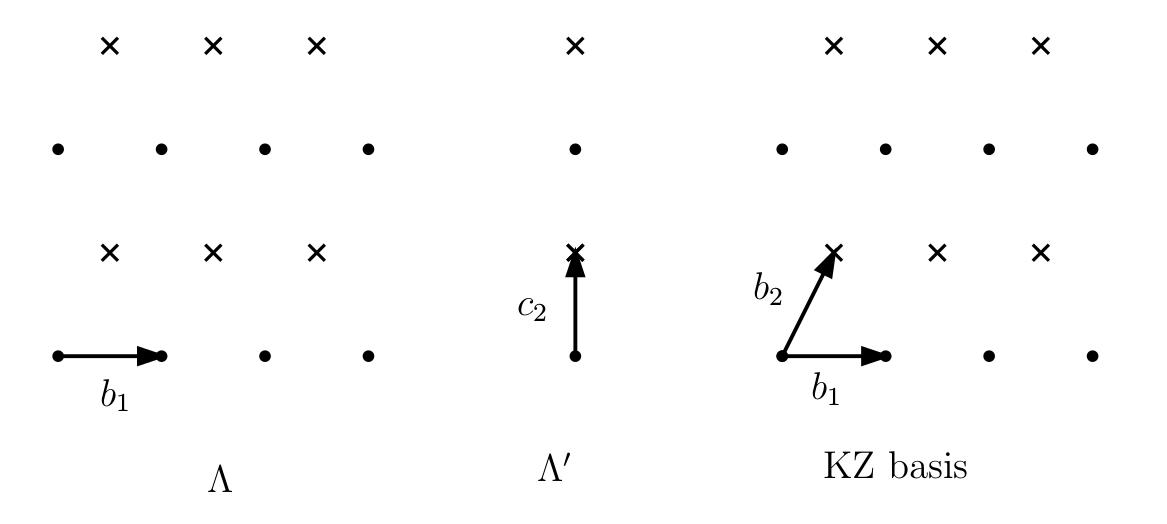
\includegraphics[width=0.8\textwidth]{Images/kzbasis.png}
  \caption{A lattice and its KZ basis}
  \label{fig:kzbasis}
\end{figure}
It is not too difficult to verify that $\Lambda'$ is indeed a lattice.
Moreover, $b_1$ is a primitive vector in $\Lambda$ (since it is a shortest
vector) and hence the vectors $b_1,\dots,b_n$ defined above indeed former
a basis of $\Lambda$. The deffinition is illustrated in \ref{fig:kzbasis}.
\par As a first application of KZ bases, we prove the following lemma by
Lagarias, Lenstra and Schnorr. Recall that for any basis, $b_1,\dots,b_n$, we 
have that
$\mathrm{min}(||\tilde{b}_1||,\dots,||\tilde{b}_n||)\leq\lambda_1(\Lambda).$
The lemma says that any lattice has a basis where this lower bound is not far 
from being tight.
\begin{lemma}[Lagarias, Lenstra, Schnorr]
  For any lattice $\Lambda$, there exists a basis $b_1,\dots,b_n$ such that
  \begin{equation}
    \mathrm{span}(||\tilde{b}_1||,\dots,||\tilde{b}_n||)\geq
    \frac{1}{n}\cdot\lambda_1(\Lambda)
  \end{equation}
\end{lemma}
\begin{proof}
  Let $d_1,\dots,d_n$ be a KZ basis of $\Lambda^*$ and let $b_n\dots,b_1$ be
  its dual basis in reverse order. We claim that $b_n,\dots,b_1$ satisfies the
  lemma. By \ref{prop:gramshmidt}, we know that $\tilde{b}_i
  = \frac{\tilde{d}_i}{||\tilde{d_i}||^2}.$ Hence, its enough to show
  that
  $\mathrm{max}(||\tilde{d}_1||,\dots,||\tilde{d}_n||)\leq\frac{n}{\lambda_1(\Lambda)}$.
  First, $\tilde{d}_1$ is the shortest vector in $\Lambda^*$. By
  \ref{prop:transference}, we have
  $||\tilde{d}_1||\leq\frac{n}{\lambda_1(\Lambda)}$. Next, $\tilde{d}_2
  = \pi_2(d_2)$ is the shortest vector in
  $\mathcal{L}(\pi_2(d_2),\dots,\pi_2(d_n))$. By \ref{prop:dualbases}, the
  dual of this lattice is $\mathcal{L}(b_2,\dots,b_n).$ But
  $\lambda_1(\mathcal{L}(b_2,\dots,b_n))\geq\lambda_1(\Lambda)$(since
  $\mathcal{L}(b_2,\dots,b_n)$ is a sublattice of $\Lambda$) and hence
  \begin{equation}
    ||\tilde{d}_2|| \leq \frac{n-1}{\lambda_1(\mathcal{L}(b_1,\dots,b_n))}\leq
      \frac{n}{\lambda_1(\Lambda)}.
    \end{equation}
    We continue similarly for all $i$.
\end{proof}

We complete this chapter with the following somewhat surprising result by
Lenstra and Schnorr. Recall that Minkowski's bound says that for any lattice
$\Lambda$,
$\lambda_1(\Lambda)\leq\sqrt{n}(\mathrm{det}(\Lambda))^{\frac{1}{n}}$. However,
it is easy to see that in many cases Minkowski's bound is far from being 
tight. Nevertheless, the following lemma implies that being able to find
vectors of lenght at most $\sqrt{n}(\mathrm{det}(\Lambda))^{\frac{1}{n}}$ is 
enough to imply an $n$-approximation to SVP (shortest vector problem).
\begin{lemma}
  Assume there exists an algorithm $A$ that given a basis $B$, finds a non-zero
  vector $v\in\mathcal{L}(B)$ such that
  \begin{equation}
    ||v|| \leq f(n)\cdot(\det(\mathcal{L}(B)))^{\frac{1}{n}}
  \end{equation}
  for some non-decreasing function $f(n)$. Then, we can approximate SVP to
  within $(f(n))^2$.
\end{lemma}
\begin{proof}
  By applying $A$ to $\mathcal{L}(B)$ and $\mathcal{L}(B)^*$ we obtain
  $u\in\mathcal{L}(B), v\in\mathcal{L}(B)^*$ such that $||u||\leq
  f(n)\cdot(\det(\mathcal{L}(B)))^{\frac{1}{n}},||v||\leq
  f(n)\cdot(\det(\mathcal{L}(B)))^{-\frac{1}{n}}$. In particular,
  $||u||\cdot||v||\leq (f(n))^2$. So the result follows from the following
  lemma.
\end{proof}
\begin{lemma}
  Assume there exists an algorithm $A$ that given a basis $B$, finds non-zero
  vectors $u\in\mathcal{L}(B), v\in\mathcal{L}(B)^*$ such taht
  $||u||\cdot||v||\leq g(n)$ for some non-decreasing function $g(n)$. Then, we
  can approximate SVP to within $g(n)$.
\end{lemma}
\begin{proof}
  First, we describe a recursive procedure that given a lattice, outputs a
  set of vectors $u_1,\dots,u_n$ in $\Lambda$ and a basis $v_1,\dots,v_n$ of 
  $\Lambda^*$. The procedure is recursive. First, apply $A$ to obtain a pair
  $u_1,v_1$. Without loss of generality, we can assume that $v_1$ is primitive
  (indeed, write $v_1 =\sum a_ib_i$ and replace it by
  $v_1/\mathrm{gcd}(a_1,\dots,a_n)$). Let $\Lambda'$ be the projection of
  $\Lambda^*$ on the subspace of $\mathrm{span}(\Lambda^*)$ orthogonal to
  $v_1$. Then apply the procedure recursively to $\Lambda'$ and let
  $u_2,\dots,u_n,v_2',\dots,v_n'$ be the result. Define $v_i=
  v_i'+\alpha_iv_1$ for the unique $\alpha_i\in(-\frac{1}{2},\frac{1}{2}]$ for
  which $v_i\in\Lambda^*$. This completes the description of the procedure.
  \par It can be checked that the output of the procedure satisfies that
  $v_1,\dots,v_n$ is a basis of $\Lambda^*$ and that for all $i,
  ||u_i||\cdot||v_i||\leq g(n-i+1)\leq g(n)$. Let $b_n,\dots,b_1$ be the 
  reversed dual basis of $v_1,\dots,v_n$. Then,
  \begin{equation}
    \min||\tilde{b}_i|| = \min\frac{1}{||\tilde{v}_i||}\leq
    \frac{1}{g(n)}\min||u_i||.
  \end{equation}
  Hence,
  \begin{equation}
    \min||u_i||\leq g(n)\cdot\min||\tilde{b}_i||\leq
    g(n)\cdot\lambda_1(\Lambda)
  \end{equation}
where we used that $b_n,\dots,b_1$ is a basis of $\Lambda$. Therefore, by
outputting the shortest vector among $u_1,\dots,u_n$ we obtain a $g(n)$
application to SVP.
\end{proof}
